The given quadratic equation can be written in the matrix form as
\begin{align}
    \vec{x}^T\myvec{1&-\frac{3}{2}\\-\frac{3}{2}&1}\vec{x}+2\myvec{5&-5}\vec{x}+21=0\label{eq:solutions/41/ex2/eq:1}
\end{align}
Calculating the parameters,we get
\begin{align}
    \mydet{\vec{V}}=\mydet{1&-\frac{3}{2}\\-\frac{3}{2}&1}=-\frac{5}{4}
\end{align}
Since, $\mydet{\vec{V}} < 0$, therefore the given  equation represents a hyperbola.\par
The characteristic equation of $\vec{V}$ will be
\begin{align}
    \mydet{\vec{V}-\lambda\vec{I}}&=\mydet{1-\lambda&-\frac{3}{2}\\-\frac{3}{2}&1-\lambda}=0\\
    &\implies 4\lambda^2-8\lambda-5 =0 \\
   &\implies\lambda_1=\frac{5}{2},\lambda_2=-\frac{1}{2}\label{eq:solutions/41/ex2/eq 2}
\end{align}
The eigen vector $\vec{p}$ is given by
\begin{align}
 \vec{V}\vec{p}=\lambda\vec{p}
\end{align}
\begin{align}
  \implies{\vec{V}-\lambda\vec{I}} \vec{p}=0 \label{eq:solutions/41/ex2/eq 3} 
\end{align}
For $\lambda_1 = \frac{5}{2} $
\begin{align}
\vec{V}-\lambda\vec{I}= \myvec{1-\frac{5}{2}&-\frac{3}{2}\\-\frac{3}{2}&1-\frac{5}{2}}
    \end{align}
    \begin{align}
 =\myvec{-\frac{3}{2}&-\frac{3}{2}\\-\frac{3}{2}&-\frac{3}{2}}
    \end{align}
    \begin{align}
    \myvec{-\frac{3}{2}&-\frac{3}{2}\\-\frac{3}{2}&-\frac{3}{2}}\xleftrightarrow{R_2=R_2-R_1}\myvec{-\frac{3}{2}&-\frac{3}{2}\\ 0 &0}
\end{align}
 \begin{align}
    \xleftrightarrow{R_1=R_1/-\frac{3}{2}}\myvec{1&1\\ 0 &0}\label{eq:solutions/41/ex2/eq 4}
   \end{align}
Substituting \eqref{eq:solutions/41/ex2/eq 4} in \eqref{eq:solutions/41/ex2/eq 3} we get 
\begin{align}
   \vec{p_1}=\myvec{-1\\1}
\end{align}
Therefore the normalized eigen vector will be
\begin{align}
    \vec{p_1}=\myvec{-\frac{1}{\sqrt{2}}\\\frac{1}{\sqrt{2}}}
\end{align}
For $\lambda_2 = -\frac{1}{2} $
\begin{align}
\vec{V}-\lambda\vec{I}= \myvec{1+\frac{1}{2}&-\frac{3}{2}\\-\frac{3}{2}&1+\frac{1}{2}}
    \end{align}
    \begin{align}
 =\myvec{\frac{3}{2}&-\frac{3}{2}\\-\frac{3}{2}&-\frac{3}{2}}
    \end{align}
    \begin{align}
    \myvec{-\frac{3}{2}&-\frac{3}{2}\\-\frac{3}{2}&-\frac{3}{2}}\xleftrightarrow{R_2=R_2+R_1}\myvec{-\frac{3}{2}&-\frac{3}{2}\\ 0 &0}
\end{align}
 \begin{align}
    \xleftrightarrow{R_1=R_1/\frac{3}{2}}\myvec{1&-1\\ 0 &0}\label{eq:solutions/41/ex2/eq 5}
   \end{align}
Substituting \eqref{eq:solutions/41/ex2/eq 5} in \eqref{eq:solutions/41/ex2/eq 3} we get 
\begin{align}
   \vec{p_2}=\myvec{1\\1}
\end{align}
Therefore the normalized eigen vector will be
\begin{align}
    \vec{p_2}=\myvec{\frac{1}{\sqrt{2}}\\\frac{1}{\sqrt{2}}}
\end{align}
Eigen decomposition\\ 
Since $\vec{V}=\Vec {V}^T$there exists an orthogonal matrix P such that
\begin{align}
    \vec{P}\vec{P}^T=\vec{I}
\end{align}
\begin{align}
    \vec{P}\vec{V}\vec{P}^T=\vec{D}= diag\brak{\lambda_1 \lambda_2}
\end{align}
or equivalently
\begin{align}
    \vec{V}= \vec{P} \vec{D} \vec{P}^T
\end{align}
As
\begin{align}
  \vec{P}=\myvec{p_1&p_2}= \myvec{-\frac{1}{\sqrt{2}}&\frac{1}{\sqrt{2}}\\\frac{1}{\sqrt{2}}& \frac{1}{\sqrt{2}}}\\
   \vec{D}=\myvec{\lambda_1&0\\0&\lambda_2}\\
   \implies 
   \vec{D}=\myvec{\frac{5}{2}&0\\0&-\frac{1}{2}} \label{eq:solutions/41/ex2/eq 6}\\
    \vec{C}=-\vec{V}^{-1}\vec{u}\\
    \implies\vec{C} =\myvec{-\frac{4}{5}&-\frac{6}{5}\\-\frac{6}{5}&-\frac{4}{5}} \myvec{-5\\ 5}\\
   = \myvec{-2\\2}
\end{align}
$\therefore$ Centre C is given by: 
\begin{align}
  \myvec{-2\\2}
%\label{eq:solutions/41/ex2/eq 6}
 \end{align}
 Now Equation \eqref{eq:solutions/41/ex2/eq 1} can be written as
\begin{align}
    \vec{y}^T\vec{D}\vec{y}=\vec{u}^T \vec {V}^{-1}\vec {u}-\vec {f}\\
\end{align}
where y is given by:
\begin{align}
     \vec{y}= \vec{P}^T\brak{\vec{x}-\vec{c}}
\end{align}
So 
\begin{align}
   \vec{y}^T\myvec{\frac{5}{2}&0\\0&-\frac{1}{2}}\vec{y}=-1\\
   \implies \vec{y}^T\myvec{\frac{5}{2}&0\\0&-\frac{1}{2}}\vec{y}+1=0
\end{align}
\begin{figure}[ht!]
	\centering
	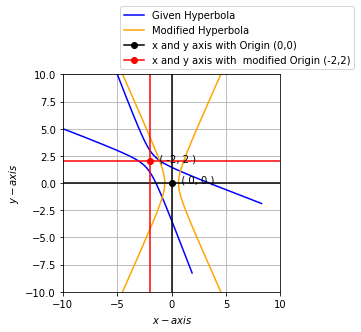
\includegraphics[width=\columnwidth]{./solutions/41/ex2/hyberbola.png}
	\caption{Hyperbola plot when origin is shifted}
	\label{eq:solutions/41/ex2/myfig}
\end{figure}
